\documentclass{imanum}
\usepackage{graphicx}

\jno{drnxxx}
\received{2018}
\revised{2018}
%\accepted{3 October 2008}

\begin{document}

\title{Link prediction using effective transition}
% Short title for running heads:
\shorttitle{Link prediction using effective transition}

\author{%
{\sc
Bryn Balls-Barker\thanks{Corresponding author. Email: bryn@mathematics.byu.edu},
Ben Webb\thanks{Email: bwebb@mathematics.byu.edu}
} \\[2pt]
Simula Research Laboratory, PO Box 134, N-1325 Lysaker, Norway and\\
Department of Informatics, University of Oslo, PO Box 1080, N-0316\\[6pt]
{\sc and}\\[6pt]
{\sc Wolfgang Hackbusch}\thanks{Email: wh@mis.mpg.de}\\[2pt]
Max Planck Institute for Mathematics in the Sciences,\\
Inselstrasse 22--26, 04103 Leipzig, Germany
}
% Short list of authors for running heads:
\shortauthorlist{B. F. Nielsen \emph{et al.}}

\maketitle

\begin{abstract}
% Body of abstract:
{Here is my abstract.}
% Keywords:
{here are some key words.}
\end{abstract}


\section{Introduction}
\label{sec;introduction}

This is an introduction to the paper. 

Background on network theory.

Background on the link prediction problem. This includes an overview of existing techniques for link prediction and some mention of how techniques work better on certain types of graphs.

Really brief into to our new method. Mention that we will walk through the derivation and algorithm, the alternate versions, and some results.

\section{Effective Transition}
\label{sec;effectivetransition}


\begin{figure}[!t]
\centering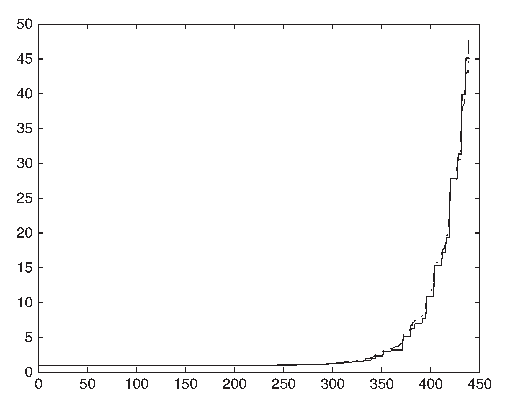
\includegraphics[scale=1.04]{fig6.eps}
\caption{The sorted array of eigenvalues
(dashed--dotted line) and of the coefficient function $k$ evaluated
at the grid points (solid line). In this case $k=k_3$ and the
mesh size is $h=0.05$.}
\label{fig:6}
\end{figure}

\begin{table}[t!]
\tblcaption{The numerical results obtained for the
generalized eigenvalue problem {\rm(\ref{atv33})} with
$k(x,y) = k_1(x,y) = 1+x+y$. In this table, as
well as in Tables {\rm\ref{table2}} and {\rm\ref{table3}},
$\lambda_j$, $\mu_j$, $h$ and $n$ represent the eigenvalue,
the value of the coefficient function evaluated at the mesh
point, the mesh width and the number of unknowns in the
discrete eigenvalue problem, respectively}
{%
\begin{tabular}{@{}ccccc@{}}
\tblhead{$h$ & $n$ & $\max_j|\lambda_j-\mu_j|$ &
$\max_j|\lambda_j -\mu_j| / h$ & Rate}
0.2\phzzz & \phzz36 & 0.1333 & 0.6667 & -- \\
0.1\phzzz & \phz121 & 0.0667 & 0.6667 & 0.9989 \\
0.05\phzz & \phz441 & 0.0333 & 0.6667 & 1.0022 \\
0.025\phz & 1681 & 0.0167 & 0.6667 & 0.9957 \\
0.0125& 6561 & 0.0083 & 0.6667 & 1.0087
\lastline
\end{tabular}
}
\label{table1}
\end{table}


\section{Operators defined on Sobolev spaces}
\label{sec;Sobolev}

In this section we will study some properties of a generalized
eigenvalue problem of the following form: find a number
$\lambda$ and a function $u$ such that
\begin{equation}
\nabla \cdot (k \nabla u) = \lambda\Delta u
\quad \hbox{in}\ \Omega.
\label{A0}
\end{equation}
Our aim is to analyse this equation in terms of operators defined on
Sobolev spaces.

To this end, let us consider a prototypical elliptic boundary-value
problem of the form
\begin{equation}
\begin{aligned}
-\nabla \cdot (k \nabla v) &= f \quad \hbox{in}\ \Omega, \\[3pt]
v &= 0 \quad \hbox{on}\ \partial \Omega,
\end{aligned}
\label{A1}
\end{equation}
where $\Omega$, with boundary $\partial \Omega$, is some open Lipschitz
domain contained in a Euclidean space $\mathbb{R}^n$. In addition, $k$
is assumed to be a uniformly positive and bounded function defined on $\Omega$, i.e.,
\begin{gather}
k \in L^{\infty}(\Omega),
\label{A2} \\[3pt]
0<b \leq k(x) \leq B \quad \hbox{for all}\ x \in \Omega ,
\label{A3}
\end{gather}
where $b$ and $B$ are given positive constants.

Throughout this section we will, for the sake of easy notation,
consider elliptic PDEs with homogeneous Dirichlet boundary conditions
(cf. (\ref{A1})). However, it is not difficult to modify the arguments
presented below to also cover cases involving Neumann conditions.


\subsection{Notation}
\label{sec3.1}

Let $H^1_0(\Omega)$, with inner product $(\cdot,\cdot)_1$ and norm
$\Vert {\cdot}\Vert_{H^1(\Omega)}$, denote the classical Sobolev
space of functions defined on $\Omega$ with zero trace at
$\partial \Omega$. According to the Riesz representation theorem,
there exist linear operators $A,L \in \mathcal{L} (H^1_0(\Omega))$
such that
\begin{align}
(A \varphi, \psi)_1 & = \int_\Omega \nabla \psi \cdot
(k \nabla \varphi) \, \mathrm{d}x
\quad \hbox{for all}\ \psi, \varphi \in H^1_0(\Omega) ,
\label{B0} \\[4pt]
(L \varphi, \psi)_1 & = \int_\Omega \nabla \psi \cdot
\nabla \varphi \, \mathrm{d}x
\quad \hbox{for all}\ \psi, \varphi \in H^1_0(\Omega) .
\label{B1}
\end{align}

With this notation at hand, the weak form of (\ref{A1}) may be written
in the following form: find $v \in H^1_0(\Omega)$ such that
\begin{equation*}
(A v, \psi)_1 = \int_{\Omega} f \psi \, \mathrm{d}x
\quad \hbox{for all}\ \psi \in H^1_0(\Omega).
\end{equation*}
Furthermore, $L$ represents the (`weak') Laplacian defined on $H^1_0(\Omega)$.


\subsection{The analysis}
\label{sec3.2}

Inspired by our findings in Section \ref{sec;preliminary}, we will
now analyse the spectrum\footnote{Here
$I:\ H^1_0(\Omega) \rightarrow H^1_0(\Omega)$ denotes the identity
operator, i.e.,
\begin{equation*}
I \psi = \psi \quad \hbox{for all}\ \psi \in H^1_0(\Omega).
\end{equation*}}
\begin{equation*}
\mathrm{sp}(L^{-1}A) = \{\lambda \in {\bf C};\
(\lambda I-L^{-1}A) \hbox{ is not invertible} \}
\end{equation*}
of the operator
\begin{equation*}
L^{-1}A:\ H^1_0(\Omega) \rightarrow H^1_0(\Omega).
\end{equation*}

For the sake of convenience, let $K$ denote the set of points in
$\Omega$ at which the coefficient function $k$ is continuous, i.e.,
\begin{equation}
K=\{ x \in \Omega;\ k \hbox{ is continuous at}\ x \}.
\label{new1}
\end{equation}
Our main result can now be formulated as follows.

\begin{theorem}
\label{theorem1}
Let $A$ and $L$ be the operators defined in (\ref{B0})
and (\ref{B1}).
\begin{NumberedListAlpha}
\item
If (\ref{A2}) and (\ref{A3}) hold then
\begin{equation*}
k(x) \in \mathrm{sp}(L^{-1}A) \quad \hbox{for all}\ x \in K,
\end{equation*}
where $K$ is the set of points defined in (\ref{new1}).
\item
In particular, if (\ref{A3}) holds and $k$ is continuous
throughout $\Omega$, i.e.,  $k \in C(\Omega)$, then
\begin{equation*}
k(x) \in \mathrm{sp}(L^{-1}A) \quad \hbox{for all}\ x \in \Omega.
\end{equation*}
\end{NumberedListAlpha}
\end{theorem}

\begin{proof}
Let $\tilde x \in K$ be arbitrary and assume that $\tilde x$ is
such that
$\tilde \lambda = k(\tilde x) \not\in \mathrm{sp}(L^{-1}A)$.

Clearly, there exists a set of functions
$\{ v_r \}_{r \in \mathbb{R}_{+}}$
satisfying\footnote{Note that no limit of $v_r$ as $r \rightarrow 0$
is needed in this proof. Only the existence of a set of functions
satisfying (\ref{C0.01}) and (\ref{C0.1}) is required.}
\begin{gather}
\mathrm{supp}(v_r) \subset \tilde x + U_r,
\label{C0.01}\\[3pt]
\parallel\! v_r \!\parallel_{H^1(\Omega)} = 1 ,
\label{C0.1}
\end{gather}
where
\begin{equation*}
U_r = \{ {\bf z} \in \mathbb{R}^n;\ |{\bf z}| \leq r \}.
\end{equation*}
Let
\begin{equation}
u_r = (\tilde \lambda I-L^{-1}A) v_r
\quad \hbox{for}\ r \in \mathbb{R}_+.
\label{C1}
\end{equation}

Since $\tilde \lambda \not \in \mathrm{sp}(L^{-1}A)$, it
follows that $(\tilde \lambda I-L^{-1}A)$ is invertible, and we
find that
\begin{equation}
\parallel\! v_r \!\parallel_{H^1(\Omega)}
=
\parallel\! (\tilde \lambda I-L^{-1}A)^{-1} u_{r}
\!\parallel_{H^1(\Omega)}
\leq \| (\tilde \lambda I-L^{-1}A)^{-1} \|
\parallel\! u_r \!\parallel_{H^1(\Omega)} .
\label{C2}
\end{equation}

By (\ref{C1}), we have
\begin{equation*}
u_r = \tilde \lambda I v_r - L^{-1} A v_r
\end{equation*}
or
\begin{equation*}
L u_r = \tilde \lambda L v_r - A v_r .
\end{equation*}
Hence it follows that
\begin{equation*}
(L u_r,u_r)_1 = \tilde \lambda (L v_r,u_r)_1 - (A v_r,u_r)_1 ,
\end{equation*}
and then, from the definition of $L$ and $A$ and
by the fact that $\mathrm{supp} (v_r) \subset \tilde x + U_r$,
we find that
\begin{equation*}
\int_{\Omega} \nabla u_r \cdot \nabla u_r \, \mathrm{d}x =
\tilde \lambda \int_{\tilde x + U_r} \nabla u_r \cdot
\nabla v_r \, \mathrm{d}x -
\int_{\tilde x + U_r} \nabla u_r \cdot (k \nabla v_r) \, \mathrm{d}x
\end{equation*}
or
\begin{equation*}
\int_{\Omega} |\nabla u_{r}|^2 \, \mathrm{d}x =
\int_{\tilde x + U_r} \nabla u_r \cdot ([\tilde \lambda-k]
\nabla v_r) \, \mathrm{d}x .
\end{equation*}
Next, by the Cauchy--Schwarz inequality, we have
\begin{equation*}
\int_{\Omega} |\nabla u_{r}|^{2} \, \mathrm{d}x \leq
\left(\int_{\Omega} |\nabla u_{r}|^{2} \, \mathrm{d}x \right)^{1/2}
\left(\int_{\tilde x + U_r} (\tilde \lambda-k)^{2}
|\nabla v_{r}|^2 \, \mathrm{d}x \right)^{1/2} ,
\end{equation*}
and, consequently,
\begin{equation}
\left( \int_{\Omega} |\nabla u_r|^{2} \,
\mathrm{d}x \right)^{1/2} \leq
\mathrm{ess} \sup_{x \in \tilde x + U_r} |\tilde \lambda - k(x)|
\parallel\! v_r \!\parallel_{H^1(\Omega)}
= \mathrm{ess} \sup_{x \in \tilde x + U_r} |k(\tilde x) - k(x)| ,
\label{C3}
\end{equation}
where the last equality follows from (\ref{C0.1}).
Since $k$ is continuous at $\tilde x$, it follows that
\begin{equation*}
\lim_{r \rightarrow 0} \mathrm{ess}
\sup_{x \in \tilde x + U_r} |k(\tilde x) - k(x)| = 0.
\end{equation*}
From (\ref{C3}) and Poincar\'e's inequality we thus conclude that
there exists a constant $r^\ast \in \mathbb{R}_+$ such that
\begin{equation}
\parallel\! u_r \!\parallel_{H^1(\Omega)} <
\frac{1}{2 \| (\tilde \lambda I-L^{-1}A)^{-1} \|}
\quad \hbox{for all}\ r \in (0,r^\ast).
\label{new2}
\end{equation}

Finally, (\ref{C2}) and (\ref{new2}) imply that
\begin{equation*}
\parallel\! v_r \!\parallel_{H^1(\Omega)} < \frac{1}{2}
\quad \hbox{for all}\ r \in (0,r^\ast),
\end{equation*}
which is a contradiction to (\ref{C0.1}). Hence we conclude that
$k(\tilde x)$ must satisfy $k(\tilde x) \in \mathrm{sp}(L^{-1}A)$.

This completes the proof of part (a) of the theorem. Part (b) is a
trivial consequence of part (a).
\end{proof}

If $k$ is continuous then we thus conclude that the range of $k$ is indeed
contained in the spectrum of $L^{-1}A$, which is in agreement with the
results of our numerical experiments. Moreover, for
problems involving discontinuous coefficient functions, i.e.,
$k \notin C(\Omega)$, we can still conclude that $k(x)$ is an eigenvalue
for the preconditioned operator $L^{-1}A$ at every point $x$ at which
$k$ is continuous.

As mentioned in Section \ref{sec;introduction}, for elliptic equations
with coefficients with large jump discontinuities, high-quality
preconditioners can sometimes be constructed due to some clustering
effect of the eigenvalues. In the case of continuous coefficients our
investigations indicate that such an effect is not likely to occur. In
particular, if the inverse Laplacian is used as a preconditioner then
the eigenvalues will not cluster.

The proof of Theorem \ref{theorem1} is not of a constructive nature.
Formulas for the eigenfunctions are not provided. To further shed some light
onto the generalized eigenvalue problem (\ref{A0}) we will now consider
it from a distributional point of view.


\section{Generalized eigenfunctions and eigenvalues}
\label{sec;distribution}

As mentioned above, our aim is to study the eigenvalue problem
\begin{equation}
\nabla \cdot (k \nabla u) = \lambda \Delta u
\label{P0}
\end{equation}
in terms of distribution theory. More precisely, we will not only
prove that $\lambda=k(x,y)$, for all $(x,y) \in \Omega$, are
eigenvalues but also present explicit formulas for the associated
generalized eigenfunctions. As in Section \ref{sec;Sobolev}, we will
assume that $\Omega$ is an open Lipschitz domain.


\subsection{Preliminaries and notation}
\label{sec4.1}

In our analysis of this eigenvalue problem the classical mollifier
functions
\citep[see, e.g.,][]{BMar86}
will play an important role. It is defined by a non-negative and
symmetric function $\omega \in C^{\infty}(\mathbb{R})$
satisfying\footnote{The standard example of such a function is
\begin{equation*}
\omega(x)=
\begin{cases}
c \exp{((x^2-1)^{-1})} & \hbox{for}\ x \in (-1,1),\\[3pt]
0 & \hbox{for}\ |x| \geq 1 ,
\end{cases}
\end{equation*}
where $c^{-1}=\int_{-1}^1 \exp{((x^2-1)^{-1})} \, \mathrm{d}x$.}
\begin{gather*}
\int_{\mathbb{R}} \omega(x) \, \mathrm{d}x =1, \\[2pt]
\omega(x) \equiv 0 \quad \hbox{for}\ |x| \geq 1.
\end{gather*}
A family $\{ \omega_\epsilon \}_{\epsilon \in \mathbb{R}_+}$
of mollifier functions are now defined by setting
\begin{equation*}
\omega_\epsilon = \frac{1}{\epsilon} \omega
\left( \frac{x}{\epsilon} \right).
\end{equation*}
Clearly, these functions possess the following properties:
\begin{gather}
\omega_\epsilon \in C^\infty, \quad \omega_\epsilon \geq 0,
\label{P1} \\[3pt]
\omega_\epsilon(x) = \omega_\epsilon(-x),
\label{P2} \\[3pt]
\int_{\mathbb{R}} \omega_\epsilon(x) \, \mathrm{d}x =1,
\label{P3} \\[3pt]
\omega_\epsilon(x) \equiv 0 \quad \hbox{for}\ |x| \geq \epsilon,
\label{P4} \\[3pt]
\omega_\epsilon(x) \leq \frac{M}{\epsilon} \quad \hbox{and} \quad
|\omega'_\epsilon(x)| \leq \frac{M}{\epsilon^2},
\label{P5}
\end{gather}
where $M$ is a positive constant that is independent of $\epsilon$.
Next we define a family
$\{ H^\epsilon \}_{\epsilon \in \mathbb{R}_+}$
of approximate Heaviside functions
\begin{equation*}
H^\epsilon(x) = \int_{-\infty}^x \omega_\epsilon(y) \, \mathrm{d}y.
\end{equation*}
Note that
\begin{gather}
0 \leq H^\epsilon(x) \leq 1\quad \hbox{for all}\ x \in \mathbb{R},
\label{P6}\\[3pt]
H^\epsilon(x) \equiv 0 \quad \hbox{for}\ x \leq -\epsilon,
\qquad H^\epsilon(x) \equiv 1 \quad \hbox{for}\ x \geq \epsilon,
\label{P6.1}\\[3pt]
(H^\epsilon)'(x) = \omega_\epsilon(x).
\label{P7}
\end{gather}

We have not been able to characterize the (generalized)
eigenfunctions and eigenvalues satisfying (\ref{P0}) for
all smooth coefficient functions $k$. However, we have been able
to do so for a fairly large class of coefficient functions that
we now describe. To this end, we define the following family $Q$
of smooth and uniformly positive functions defined on
$\overline \Omega$:
\begin{equation*}
Q = \{k \in C^\infty (\overline \Omega );\ \exists\, m \in
\mathbb{R}_+ \hbox{ such that } m \leq k(x,y)
\hbox{ for all } (x,y) \in \overline \Omega \} .
\end{equation*}
It turns out that the generalized eigenfunctions satisfying (\ref{P0})
are characterized by the regions in the domain $\Omega$ on which
the coefficient function $k$ is constant, i.e., by the contour curves
of $k$. Therefore, for each $k \in Q$ and $(x_0,y_0) \in \Omega$, we
introduce the set
\begin{equation}
S(k,(x_0,y_0))= \{(x,y) \in \Omega ;\ k(x,y)=k(x_0,y_0)\}.
\label{P7.5}
\end{equation}

With this notation at hand, we are ready to define the set $K$ of
coefficient functions for which we are able to provide a
detailed mathematical analysis of the eigenvalue problem
(\ref{P0}) as follows:
\begin{equation}
\begin{aligned}
K & = \{ k \in Q ; \hbox{ for all } (x,y) \in \Omega,
|S(k,(x,y))|=0 \hbox{ or } S(k,(x,y)) \\
& \qquad \hbox{ contains at least one open and connected subset }
G \hbox{ with } |G| > 0 \}.
\end{aligned}
\label{P8}
\end{equation}
Here $|S(k,(x,y))|$ and $|G|$ denote the measures of the respective
sets. Roughly speaking, $K$ consists of those smooth functions that
are `well behaved' in a measure-theoretical sense.
The need for these assumptions on the coefficient function will
become apparent in the analysis below.

Clearly, the distributional form of the eigenvalue problem (\ref{P0})
can be written in the following form: find a number $\lambda$ and
a (possibly generalized) function $u$ such that
\begin{equation}
\int_\Omega k \nabla u \cdot \nabla \phi \, \mathrm{d} \Omega =
\lambda \int_\Omega \nabla u \cdot \nabla \phi \, \mathrm{d} \Omega
\quad \hbox{for all}\ \phi \in C^\infty_0(\Omega) ,
\label{P9}
\end{equation}
where $C^\infty_0(\Omega)$ denotes the set of test functions, i.e., the
set\footnote{$C^{\infty}_0(\Omega)=\{\psi \in C^{\infty}(\Omega);\
\exists\,\hbox{a compact set }K \subset \Omega \hbox{ such that }
\{x;\ \psi(x) \neq 0 \} \subset K \}$.}
of smooth functions with compact support in $\Omega$.
This means that
\begin{equation}
\int_\Omega (k-\lambda) [u_x \phi_x + u_y \phi_y] \, \mathrm{d} \Omega
= 0 \quad \hbox{for all}\ \phi \in C^\infty_0(\Omega) .
\label{P10}
\end{equation}
In the analysis below we will use the form (\ref{P10}) of the
generalized eigenvalue problem. The analysis is divided, by certain
properties of the coefficient function $k$, into three different cases.


\subsection{The analysis}
\label{sec4.2}

\subsubsection{Case I}
\label{sec4.2.1}

Let $k \in K$ and assume that $(x_0,y_0) \in \Omega$ is a point such that
\begin{gather}
k_x(x_0,y_0) \neq 0 \quad \hbox{or} \quad k_y(x_0,y_0) \neq 0,
\label{P10.1}\\[3pt]
|S(k,(x_0,y_0))| =0.
\label{P10.2}
\end{gather}
We will now study the sequence of functions
\begin{equation*}
H^{\epsilon}(k(x,y)-k_0)
\end{equation*}
for $\epsilon > 0$, where $k_0=k(x_0,y_0)$. More precisely, we will show
that $k_0$ is an eigenvalue with associated eigenfunction $H(k(x,y)-k_0)$,
where $H$ denotes the Heaviside function
\begin{equation}
H(z) =
\begin{cases}
0 & \hbox{for } z \leq 0, \\[2pt]
1 & \hbox{for } z > 0.
\end{cases}
\label{P10.3}
\end{equation}

Motivated by the discussion of the numerical experiments above
and the form (\ref{P10}) of the generalized eigenvalue problem, we
will, for an arbitrary test function $\phi \in C^\infty_0(\Omega)$,
study the integral
\begin{align}
I_\epsilon &= \int_\Omega (k-k_0) [H^\epsilon_x(k-k_0) \phi_x
+ H^\epsilon_y(k-k_0) \phi_y] \, \mathrm{d} \Omega \notag\\[3pt]
&= \int_\Omega (k-k_0) [k_x \omega_\epsilon (k-k_0) \phi_x +
k_y \omega_\epsilon (k-k_0) \phi_y] \, \mathrm{d} \Omega.
\label{P11}
\end{align}
If we apply the property (\ref{P4}) of the mollifier and define
\begin{equation}
S_{\epsilon}= \{(x,y) \in \Omega;\ |k(x,y)-k(x_0,y_0)| < \epsilon \}
\label{P12}
\end{equation}
then we find that
\begin{equation*}
I_\epsilon = \int_{S_\epsilon}
(k-k_0) [k_x \omega_\epsilon(k-k_0) \phi_x +
k_y \omega_\epsilon (k-k_0) \phi_y] \, \mathrm{d} \Omega.
\end{equation*}
Next, since $k_x, k_y, \phi_x, \phi_y \in L_{\infty}(\Omega)$,
property (\ref{P5}) of the mollifier function $\omega_\epsilon$ and
the triangle inequality imply the existence of a positive constant
$c_1$, independent of $\epsilon$, such that
\begin{align*}
|I_\epsilon| & \leq \int_{S_\epsilon}
|k-k_0| [|k_x \omega_\epsilon(k-k_0) \phi_x| +
|k_y \omega_\epsilon(k-k_0) \phi_y|] \, \mathrm{d} \Omega \\[3pt]
& \leq \int_{S_\epsilon} |k-k_0| [
\parallel\! k_x \!\parallel_\infty
\parallel\! \phi_x \!\parallel_\infty
M \epsilon^{-1} +
\parallel\! k_y \!\parallel_\infty
\parallel\! \phi_y \!\parallel_\infty
M \epsilon^{-1}] \, \mathrm{d} \Omega \\[3pt]
& \leq  c_1 \int_{S_{\epsilon}}
|k-k_0| \epsilon^{-1} \, \mathrm{d} \Omega.
\end{align*}
However, on the set $S_\epsilon$ (see (\ref{P12}))
we have $|k-k_0| < \epsilon$ and we therefore conclude that
\begin{equation}
|I_\epsilon| \leq c_1 \int_{S_\epsilon} 1 \, \mathrm{d} \Omega =
c_1 |S_\epsilon|,
\label{P13}
\end{equation}
where $|S_\epsilon|$ denotes the measure of $S_\epsilon$.
Recall the definitions (\ref{P7.5}) and (\ref{P12}) of $S(k,(x_0,y_0))$
and $S_\epsilon$, respectively. Clearly,
\begin{equation*}
\bigcap_{\epsilon > 0} S_\epsilon = S(k,(x_0,y_0)),
\end{equation*}
and it is therefore natural to ask if the measure of $S_\epsilon$
converges toward the measure of $S(k,(x_0,y_0))$ as
$\epsilon \rightarrow 0$. This question is treated in detail in
Appendix A and the answer to it is affirmative
(see Lemma \ref{lemma1}).
Thus assumption (\ref{P10.2}) implies that
\begin{equation*}
\lim_{\epsilon \rightarrow 0} |S_\epsilon| =0,
\end{equation*}
and we conclude that
\begin{equation}
\lim_{\epsilon \rightarrow 0} |I_\epsilon| =0.
\label{P14}
\end{equation}

Having established that the integral defined in (\ref{P11}) tends
toward zero as $\epsilon \rightarrow 0$, we must now check whether
or not the sequence of functions
$\{ H^{\epsilon}(k-k_0) \}_{\epsilon \in \mathbb{R}_+}$ has a well-defined,
in the distributional sense, limit as $\epsilon \rightarrow 0$. More
precisely, we will show, as expected, that $H(k-k_0)$ is the limit.
To this end, consider for an arbitrary test function
$\phi \in C^{\infty}_0$ the integral
\begin{align*}
D_\epsilon &= \int_\Omega H^\epsilon (k-k_0) \phi \, \mathrm{d} \Omega
- \int_\Omega H(k-k_0) \phi \, \mathrm{d} \Omega \\[3pt]
&= \int_\Omega [H^\epsilon (k-k_0)- H(k-k_0)] \phi \, \mathrm{d} \Omega.
\end{align*}
From the property (\ref{P6.1}) of the approximate Heaviside function
$H^\epsilon$ we find that
\begin{equation*}
H^\epsilon (k-k_0) = H(k-k_0)  \quad \hbox{for all}\ (x,y)
\hbox{ such that }|k(x,y)-k_0| \geq \epsilon.
\end{equation*}
Hence
\begin{equation*}
D_\epsilon = \int_{S_\epsilon}
[H^\epsilon (k-k_0)- H(k-k_0)] \phi \, \mathrm{d} \Omega,
\end{equation*}
and then the property (\ref{P6}) and the definition (\ref{P10.3}) of
the Heaviside function imply that
\begin{equation*}
|D_\epsilon| \leq
\parallel\! \phi \!\parallel_\infty
\int_{S_{\epsilon}} \, \mathrm{d} \Omega =
\parallel\! \phi \!\parallel_\infty |S_\epsilon| .
\end{equation*}
As discussed above, $|S_\epsilon| \rightarrow 0$ as
$\epsilon \rightarrow 0$, and we conclude that
\begin{equation*}
\lim_{\epsilon \rightarrow 0}H^\epsilon (k-k_0) = H(k-k_0)
\end{equation*}
in the distributional sense. From standard theory
\citep[see][]{BGri81},
for the derivatives of distributions, it follows that
\begin{equation*}
\lim_{\epsilon \rightarrow 0}H^\epsilon_x (k-k_0)
= H_x(k-k_0),
\quad  \lim_{\epsilon \rightarrow 0}H^\epsilon_y (k-k_0)
= H_y(k-k_0).
\end{equation*}

Finally, by combining these convergence properties of the approximate
Heaviside functions and (\ref{P11}) and (\ref{P14}) we find that
\begin{equation*}
\int_\Omega k \nabla H(k-k_0) \cdot \nabla \phi \, \mathrm{d} \Omega =
k_0 \int_\Omega \nabla H(k-k_0) \cdot \nabla \phi \, \mathrm{d} \Omega
\quad \hbox{for all}\ \phi \in C^\infty_0 .
\end{equation*}

Note that (\ref{P10.1}) ensures that $H(k-k_0) \neq 0$, and thus,
if $k$ satisfies (\ref{P10.1}) and (\ref{P10.2}) then
$H(k(x,y)-k_0)$ is an eigenfunction, in the distributional sense, with
associated eigenvalue $k_0=k(x_0,y_0)$ for the generalized eigenvalue
problem (\ref{P0}).

The next question is, of course, what happens if either assumption
(\ref{P10.1}) or (\ref{P10.2}) fails to hold? This is the topic of
Sections \ref{sec4.2.2} and \ref{sec4.2.3}.


\subsubsection{Case II}
\label{sec4.2.2}

Let $k \in K$ and assume that $(x_0,y_0) \in \Omega$ is a point such that
\begin{equation}
k_x(x_0,y_0) = 0 \quad \hbox{and} \quad k_y(x_0,y_0) = 0.
\label{Pc1}
\end{equation}
In this case we will show that the Dirac delta function is an
eigenfunction, in the distributional sense, for the generalized
eigenvalue problem (\ref{P9}).

To this end, let $\delta$ denote the delta distribution associated
with the point $(x_0,y_0)$, i.e., $\delta$ denotes the linear functional
\begin{equation*}
\delta:\ C^{\infty}_0 \rightarrow \mathbb{R}
\end{equation*}
such that the action of applying $\delta$ to $\phi \in C^\infty_0$ is
given by
\begin{equation}
\langle \delta,\phi \rangle = \phi(x_0,y_0).
\label{Pc1.1}
\end{equation}
Note that we use the notation
\begin{equation*}
\langle \delta,\phi \rangle = \int_\Omega \delta \phi\,
\mathrm{d} \Omega = \phi(x_0,y_0).
\end{equation*}

Recall the form (\ref{P9}) of the eigenvalue problem. Let
$\phi \in C^\infty_0$ be an arbitrary test function and consider
the integral
\begin{equation*}
I_1 = \int_\Omega k \nabla \delta \cdot \nabla \phi\, \mathrm{d} \Omega =
\int_\Omega ( k \delta_x \phi_x + k \delta_y \phi_y ) \,
\mathrm{d} \Omega.
\end{equation*}
Now integration by parts implies that
\begin{align*}
I_1 &= - \int_\Omega (\delta [k_x \phi_x+k \phi_{xx}]
+ \delta [k_y \phi_y+k \phi_{yy}]{)} \, \mathrm{d} \Omega \\[3pt]
&= - [k_x(x_0,y_0) \phi_x(x_0,y_0)+k(x_0,y_0) \phi_{xx}(x_0,y_0)
+ k_y(x_0,y_0) \phi_y(x_0,y_0)+k(x_0,y_0) \phi_{yy}(x_0,y_0)] \\[3pt]
&= - [k(x_0,y_0) \phi_{xx}(x_0,y_0)+k(x_0,y_0) \phi_{yy}(x_0,y_0)],
\end{align*}
where the last equality follows from assumption (\ref{Pc1}).
On the other hand, by inserting $\lambda=k_0=k(x_0,y_0)$ and $u=\delta$
in the right-hand side of (\ref{P9}) we find that
\begin{align*}
I_2 &= k_0 \int_\Omega \nabla \delta \cdot \nabla \phi \,
\mathrm{d} \Omega
= k_0 \int_\Omega (\delta_x \phi_x + \delta_y \phi_y) \,
\mathrm{d} \Omega \\[3pt]
&= - k_0 \int_\Omega (\delta \phi_{xx} + \delta \phi_{yy}) \,
\mathrm{d} \Omega\\[3pt]
&= - k(x_0,y_0) [\phi_{xx}(x_0,y_0)+ \phi_{yy}(x_0,y_0)].
\end{align*}
Thus $I_1=I_2$ and it follows that the $\delta$-distribution associated
with the point $(x_0,y_0)$ is an `eigenfunction' with eigenvalue
$k(x_0,y_0)$, provided that (\ref{Pc1}) holds.


\subsubsection{Case III}
\label{sec4.2.3}

Let $k \in K$ and assume that $(x_0,y_0) \in \Omega$ is a point
such that
\begin{equation}
|S(k,(x_0,y_0))| > 0
\label{Pc2}
\end{equation}
(cf. (\ref{P7.5}) and (\ref{P8})).
This is, in fact, the simplest case. According to the definition
of $K$ in (\ref{P8}), $S(k,(x_0,y_0))$ contains an open and connected subset
$G$ with strictly positive measure, i.e., $|G|>0$. This ensures the
existence of nonzero functions whose support is contained in $G$.
Let $u$ be such a function, i.e., we assume that
\begin{equation}
\mathrm{supp}(u) \subset G.
\label{Pc3}
\end{equation}
Since $k(x,y) = k(x_0,y_0)$ on $G$, it follows that
\begin{align*}
\int_\Omega k \nabla u \cdot \nabla \phi\, \mathrm{d} \Omega &=
k(x_0,y_0) \int_G \nabla u \cdot \nabla \phi\,
\mathrm{d} \Omega \\[3pt]
&= k(x_0,y_0) \int_\Omega \nabla u \cdot \nabla \phi \,
\mathrm{d} \Omega,
\end{align*}
which should be compared with (\ref{P9}). Hence we conclude
that in this case every nonzero function satisfying (\ref{Pc3})
is a generalized eigenfunction with associated eigenvalue
$k(x_0,y_0)$.

\begin{theorem}
Let $k$ be a coefficient function in the set $K$ defined in (\ref{P8}).
For every $(x_0,y_0) \in \Omega$ there exists a generalized function
$u$ such that $\lambda=k(x_0,y_0)$ and $u$ forms an
eigenvalue--eigenfunction pair for the generalized eigenvalue
problem (\ref{P0}).

Furthermore, the following statements hold.
\begin{BulletedList}
\item
If conditions (\ref{P10.1}) and (\ref{P10.2}) hold then
\begin{equation*}
u=H(k-k_0)
\end{equation*}
is an eigenfunction with associated eigenvalue
$\lambda = k_0 = k(x_0,y_0)$. Here $H$ denotes the Heaviside
function (see (\ref{P10.3})).

\item
If condition (\ref{Pc1}) holds then
\begin{equation*}
u=\delta_{(x_0,y_0)}
\end{equation*}
is a generalized eigenfunction with associated eigenvalue
$\lambda = k_0 = k(x_0,y_0)$. Here $\delta_{(x_0,y_0)}$ is
the Dirac delta distribution associated with the point
$(x_0,y_0)$ (see (\ref{Pc1.1})).

\item
If condition (\ref{Pc2}) holds then any function $u$ satisfying
(\ref{Pc3}), where $G$ is the set defined in (\ref{P8}), is a solution
of the generalized eigenvalue problem (\ref{P0}) with associated
eigenvalue $\lambda = k_0 = k(x_0,y_0)$.
\end{BulletedList}
\end{theorem}


\section{Conclusions}
\label{sec5}

In this paper we have analysed the eigenvalues and eigenfunctions of
second-order elliptic PDEs preconditioned by the inverse of the
Laplacian. We have shown by numerical experiments and mathematical
analysis that there is a strong relation between the spectrum of
the preconditioned operator and the range of the coefficient
function $k$, provided that $k$ is smooth and satisfies certain
measure-theoretical properties.

More precisely, in the discrete case the spectrum seems to be
accurately approximated by the values of the coefficient function
evaluated at the mesh points. Furthermore, we have proven, both
for the associated operators defined on Sobolev spaces and in terms
of generalized functions, that the range of $k$ is contained in
the spectrum of the preconditioned operator.

The purpose of this paper has been to obtain a deeper understanding
of the convergence properties of the CG method applied to
second-order elliptic equations. For problems with large jump
discontinuities in the coefficients the success of efficient
preconditioners is commonly based on some sort of clustering effect
of the eigenvalues. The present work shows that such an approach might
be very difficult to apply to problems involving continuous
coefficients with large variations. In particular, if the inverse
Laplacian is applied as a preconditioner then such a clustering effect
will not occur.


\section*{Acknowledgements}

We would like to thank Kent-Andre Mardal for helping us with the
implementation of the C++ software used in this work. Furthermore, we
are very grateful to the referees for their most interesting comments
and suggestions.


\bibliographystyle{IMANUM-BIB}
\bibliography{IMANUM-refs}

\clearpage

\appendix


\section*{Appendix A.\ A measure-theoretical lemma}
\label{app1}

Let $k:\ \Omega \rightarrow \mathbb{R}$ be a measurable function,
let $(x_0,y_0)$ be an arbitrary point in $\Omega$ and consider
the sets
\begin{align}
S_0 & = \{ (x,y) \in \Omega;\ k(x,y) = k(x_0,y_0) \},
\label{Ap1}
\\[4pt]
S_\epsilon & = \{ (x,y) \in \Omega;\ |k(x,y) - k(x_0,y_0)|
\leq \epsilon \}.
\label{Ap2}
\end{align}
Note that
\begin{equation}
S_0 \subset S_\epsilon \quad \hbox{for all}\ \epsilon > 0,
\label{Ap3}
\end{equation}
and, furthermore,
\begin{equation*}
\bigcap_{\epsilon > 0} S_{\epsilon} = S_0.
\end{equation*}
Motivated by these properties, we now establish the following lemma.

\begin{lemma}
\label{lemma1}
Let $k:\Omega \rightarrow \mathbb{R}$ be a measurable function and
let $S_0$ and $S_\epsilon$ denote the sets defined in (\ref{Ap1})
and (\ref{Ap2}), respectively. If the area of $\Omega$ is finite,
i.e., $|\Omega| < \infty$, then
\begin{equation*}
\lim_{\epsilon \rightarrow 0} |S_\epsilon| = |S_0|,
\end{equation*}
where $|S_0|$ and $|S_\epsilon|$ denote the measures of these sets.
\end{lemma}

\begin{proof}
Let $\mathcal{X}_0$ and $\mathcal{X}_\epsilon$ denote the
characteristic functions of $S_0$ and $S_\epsilon$, respectively,
that is,
\begin{equation*}
\mathcal{X}_0 (x,y) =
\begin{cases}
1 & \hbox{for } (x,y) \in S_0, \\[2pt]
0 & \hbox{elsewhere}
\end{cases}
\end{equation*}
and
\begin{equation*}
\mathcal{X}_\epsilon (x,y) =
\begin{cases}
1 & \hbox{for } (x,y) \in S_\epsilon, \\[2pt]
0 & \hbox{elsewhere}.
\end{cases}
\end{equation*}

We start by proving that $\mathcal{X}_\epsilon$ converges point-wise
toward $\mathcal{X}_0$ as $\epsilon \rightarrow 0$. Let
$(\tilde x, \tilde y)$ be an arbitrary point in $\Omega$.
\begin{NumberedListAlpha}
\item
If $(\tilde x, \tilde y) \in S_0$ then (\ref{Ap3}) implies that
\begin{equation*}
\mathcal{X}_0 (\tilde x, \tilde y) = 1 =
\mathcal{X}_\epsilon (\tilde x, \tilde y)
\quad \hbox{for all}\ \epsilon > 0.
\end{equation*}

\item
If $(\tilde x, \tilde y) \notin S_0$ then
\begin{equation*}
\mathcal{X}_0 (\tilde x, \tilde y) = 0.
\end{equation*}
\end{NumberedListAlpha}
Moreover, for $\epsilon < |k(\tilde x, \tilde y) - k(x_0,y_0)|$
it follows from the definition (\ref{Ap2}) of $S_\epsilon$
that $(\tilde x, \tilde y) \notin S_\epsilon$. Hence
\begin{equation*}
\mathcal{X}_\epsilon (\tilde x, \tilde y) = 0
\quad \hbox{for all}\ \epsilon
< |k(\tilde x, \tilde y) - k(x_0,y_0)|.
\end{equation*}
Clearly, (a) and (b) imply that
\begin{equation*}
\lim_{\epsilon \rightarrow 0} \mathcal{X}_\epsilon
(\tilde x, \tilde y)
= \mathcal{X}_0 (\tilde x, \tilde y) ,
\end{equation*}
and we conclude that $\mathcal{X}_\epsilon$ converges point-wise
toward $\mathcal{X}_0$ as $\epsilon \rightarrow 0$.

Note that (cf. (\ref{Ap3}))
\begin{equation*}
|1-\mathcal{X}_\epsilon| = 1 - \mathcal{X}_\epsilon
\leq 1 - \mathcal{X}_0
\quad \hbox{for all}\ \epsilon > 0.
\end{equation*}
Thus the dominated convergence theorem
\citep[see, e.g.,][]{BRoy89}
implies that
\begin{equation*}
\lim_{\epsilon \rightarrow 0} \int_\Omega
(1-\mathcal{X}_\epsilon) \, \mathrm{d} \Omega
= \int_\Omega (1-\mathcal{X}_0) \, \mathrm{d} \Omega.
\end{equation*}
Consequently, since $\Omega$ has a finite measure,
\begin{equation*}
\lim_{\epsilon \rightarrow 0} |S_\epsilon| = |S_0|,
\end{equation*}
which finishes the proof.
\end{proof}
\end{document}
